\section{Privilege escalation to \LoginName{root}.}
\par We begin our new enumeration step by reading \UserName{steven}'s mails: he has one, reported in listing \ref{undetected_mail}.
\begin{listing}
  \small
  \input{mail}
  \caption{\MachineName{Undetected}: \UserName{steven}'s mail.}
  \label{undetected_mail}
\end{listing}
\par We learn that something is wrong with the \ServiceName{Apache} service: this is then where we are going to look next. Inspecting the files in \FileName{/etc/apache2/mods-available}, we see that all files are identified by the \SoftwareName{file} utility as ``ASCII text'', expect one called \FileName{mod\_reader.o} which is ``ELF 64-bit LSB relocatables'' instead . Using \mintinline{bash}{ls -l} we also remark that \FileName{mod\_reader.o} is one of the few files that have not been last modified on April 13th.
\par Just as before, we download it on our attacking machine to inspect it with strings: again, we find a mysterious string a bit long. This time, it does not look as an hexadecimal number, but we remark that all the characters used are typical of base64 encoding: we then try to decode it as base64 and we are successful, see listings \ref{undetected_decode-mod_reader-payload.sh} and \ref{undetected_mod_reader-payload.sh}.
\begin{listing}
  \insertcode{bash}{decode-mod_reader-payload.sh}
  \caption{\MachineName{Undetected}: Command to decode the base64 encoded string found in \FileName{mod\_reader.o} and placed into the \mintinline{bash}{BASE64_STRING} variable.}
  \label{undetected_decode-mod_reader-payload.sh}
\end{listing}
\begin{listing}
  \tiny
  \insertcode{bash}{mod_reader-payload.sh}
  \caption{\MachineName{Undetected}: Commands encoded into \FileName{mod\_reader.o} and retrieved through listing \ref{undetected_decode-mod_reader-payload.sh}.}
  \label{undetected_mod_reader-payload.sh}
\end{listing}
\par The commands we just decoded are very odd: it looks like an image is downloaded and saved as a binary in \FileName{/usr/sbin} called \FileName{sshd}, which is normally the name of an \ServiceName{ssh} daemon. Moreover, its last time modified date is overwritten and set artificially to the same date \FileName{/usr/sbin/a2enmod} was last modified: this looks much as an attempt to download malware on the machine and hide it.
\par We download \FileName{/usr/sbin/sshd} on our machine and decompile it using \SoftwareName{ghidra}. In the \FunctionName{auth\_password} function (figure \ref{undetected_sshd.png}), thanks to the fact that the binary is not stripped, we remark the presence of an array called \VariableName{backdoor} which seems to contain an obfuscated string that can be used as a password.
\begin{figure}
        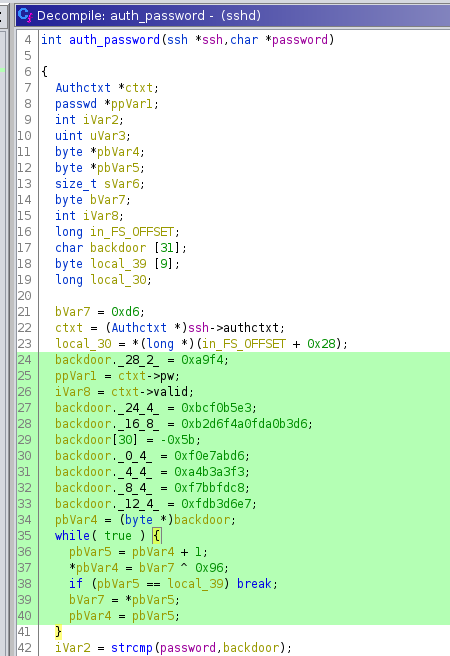
\includegraphics[width=0.75\textwidth]{sshd.png}
        \centering
        \caption{\MachineName{Undetected}: Definition and use of the \VariableName{backdoor} array.}
        \label{undetected_sshd.png}
\end{figure}
\par We write a quick \LanguageName{python} script to deobfuscate the backdoor password, see listings \ref{undetected_build-backdoor.py} and \ref{undetected_backdoor}.
\begin{listing}
  \insertcode{python}{build-backdoor.py}
  \caption{\MachineName{Undetected}: \LanguageName{Python} script to deobfuscate the backdoor password.}
  \label{undetected_build-backdoor.py}
\end{listing}
\begin{listing}
  \input{backdoor}
  \caption{\MachineName{Undetected}: Output of the script in listing \ref{undetected_build-backdoor.py}.}
  \label{undetected_backdoor}
\end{listing}
\par Logging as \LoginName{root} through \SoftwareName{ssh} with the password in listing \ref{undetected_backdoor}, we get indeed \LoginName{root} access to the machine.
